\documentclass[a4paper,titlepage,11pt]{article}

\usepackage[top=2.54cm, bottom=2.54cm, left=2.54cm, right=2.54cm]{geometry}
\usepackage[utf8x]{inputenc}
\usepackage{hyperref}
\usepackage{graphicx}
\usepackage{hyperref}
\usepackage{multicol}
\usepackage{textcomp, xspace}

\begin{document}

\begin{titlepage}
  \begin{center}
    {\scshape \huge Graph Library \par}
    \vspace{1cm}

    {\scshape \LARGE Project \par}
    \vspace{1.5cm}

    {\scshape \Large Complex Network \par}
    \vspace{0.5cm}

    {\Large Alameda \par}
    \vfill

    {\itshape \Large Group 6 \par}
    \vfill

    \begin{tabular}{l l}
      Bernardo Casaleiro & 87827\\
      João Godinho & 87830\\
    \end{tabular}
    \vfill

    {\large \today\par}
  \end{center}
\end{titlepage}

\section{Introduction}
As students coming from Computer Science we thought that the development of a small library for the third topic of the project would be interesting.
So we developed a simple library that generates a graph. This can be done randomly, using the random model or the Barabási-Albert model, or as '.gml' file.

After the graph is obtained you can use the available graph class attributes and methods as described below.

We chose \href{https://www.python.org}{Python} as our programming language for its simplicity and great comunity in this field.
For parsing the data sets we used the \href{https://networkx.github.io}{networkx} library, only using it to read the  '.gml' files and to receive the list of nodes and their edges.

In our implementation we assumed that the graphs are not directed.

\section{Library Structure}
In our library we tried to fight Python's speed problem. So we avoid any type of re-calculations.
In every method we first check if the graph has already that attribute set.
If it doesn't it's calculated and loaded into the respective atribute. Otherwise the method simply returns the attribute.

Because of that we advise the use of the \textit{get} methods for each variable.

\subsection*{Classes}
\begin{description}
\item [graph] Graph class where all the information of the graph is kept

\textit{ \textbf{Attributes} }
\begin{description}
\item [ nodes ] array:node \textbf{-} list of nodes
\item [ adjancy\_matrix ] array:array:int \textbf{-} adjacency matrix
\item [ clustering\_coefficient ] float \textbf{-} clustering coefficient
\item [ average\_path\_length ] float \textbf{-} average path length
\item [ max\_node\_degree ] int \textbf{-} maximum node degree in the graph
\item [ degree\_histogram ] array:int \textbf{-} degree histogram
\item [ degree\_distribution ] array:float \textbf{-} degree distribution
\item [ comulative\_degree\_distribution ] array:float \textbf{-} comulative degree distribution
\end{description}

\textit{ \textbf{Methods} }
\begin{description}
\item [get\_nodes] array:node ( ) - returns the list of nodes
\item [get\_adjacency\_matrix] array:array:int ( ) \textbf{-} returns the adjacency matrix
\item [get\_clustering\_coefficient] float ( ) \textbf{-} returns the clustering coefficient
\item [get\_average\_path\_length] float ( ) \textbf{-} returns the average path length
\item [calc\_node\_degrees] void ( ) \textbf{-} calculates the node degree for each node
\item [get\_max\_node\_degree] int ( ) \textbf{-} returns the maximum node degree in the graph
\item [get\_node\_degree\_histogram] array:int ( ) \textbf{-} returns the degree histogram
\item [get\_degree\_distribution] array:float ( ) \textbf{-} returns the degree distribution
\item [get\_cumulative\_degree\_distribution] array:float ( ) \textbf{-} returns the comulative degree distribution
\end{description}

\item [node] Node class where all the information of each node is kept

\textit{ \textbf{Atributes} }
\begin{description}
\item [edges] array:edge \textbf{-} list of the edges
\item [degree] int \textbf{-} degree of the node
\end{description}

\textit{ \textbf{Methods} }
\begin{description}
\item [get\_edges] array:edge ( ) \textbf{-} returns the list of edges
\item [get\_node\_degree] int ( ) \textbf{-} returns the node degree
\end{description}

\item [edge] Edge class where all the information of each edge is kept

\textit{ \textbf{Atributes} }
\begin{description}
\item [source] int \textbf{-} index of the source node
\item [target] int \textbf{-} index of the target node
\end{description}

\textit{ \textbf{Methods} }
\begin{description}
\item [get\_source] int ( ) \textbf{-} returns the source node
\item [get\_target] int ( ) \textbf{-} returns the target node
\end{description}

\end{description}

\subsection*{Methods}
\begin{description}
\item [read\_file] graph (string) \textbf{-} reads a proper formated gml file returning the graph object for that file
\item [generate\_random\_graph] graph (number of nodes, prob) \textbf{-} receives a number of nodes and the probability of
                                                            having a link between each other returning a random graph with that parameters
\item [generate\_minimal\_model] graph (number of initial nodes, number of nodes) \textbf{-} receives the number of initial nodes that the 																graph will be initialized and the number of nodes that will be inserted on 																 the graph returning a random graph
\item [bfs] int (adjacency matrix, origin, destiny) \textbf{-} returns the shortest distance between node origin and destiny
\item [floyd\_warshall] array:array:int (adjacency matrix) \textbf{-} returns shortest distance between all nodes in the graph

\end{description}

\newpage

\section{Results}
\subsection{Dataset}
\subsubsection{power.gml}
Network representing the topology of the Western States Power Grid of the United States.

\begin{figure}[h]
    \centering
    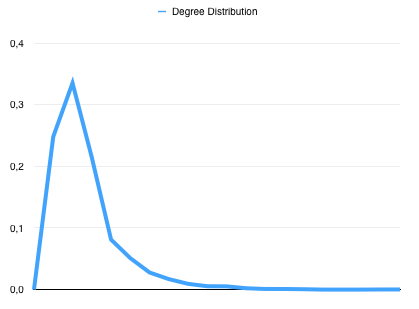
\includegraphics[scale=0.50]{img/dd-dataset.png}
    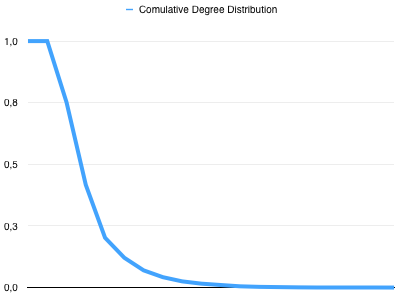
\includegraphics[scale=0.50]{img/cdd-dataset.png}
\end{figure}

\begin{multicols}{2}

  \textbf{Clustering Coefficient}

  0,08010

\columnbreak

  \textbf{Average Path Length}

  18,98918


\end{multicols}

\subsection{Random Graph}

\begin{figure}[h]
    \centering
    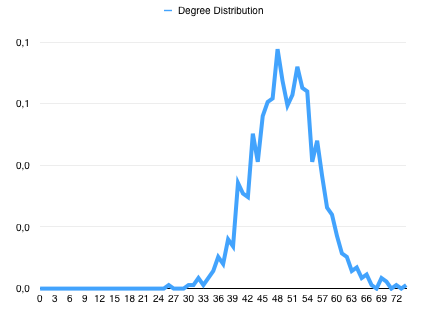
\includegraphics[scale=0.50]{img/dd-1000-05.png}
    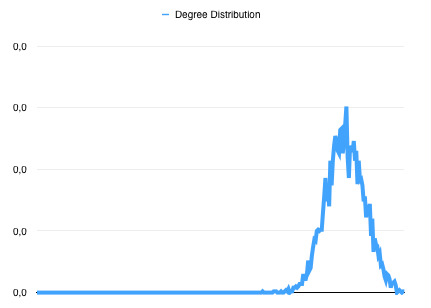
\includegraphics[scale=0.50]{img/dd-5000-05.png}
\end{figure} 


\textbf{Comulative Degree Distribution}

\begin{figure}[h]
    \centering
    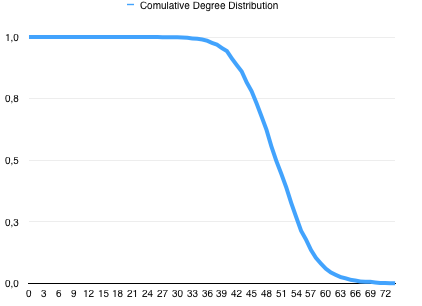
\includegraphics[scale=0.50]{img/cdd-1000-05.png}
    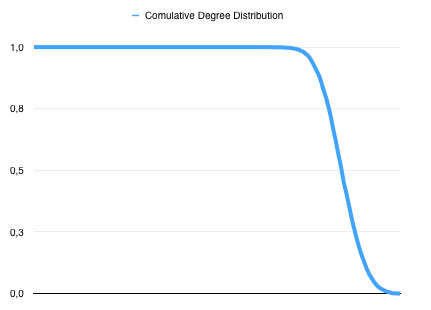
\includegraphics[scale=0.50]{img/cdd-5000-05.png}
\end{figure}

\begin{multicols}{2}

  \textbf{Clustering Coefficient}

  \textbf{(nodes=1000,p=0.05)} 0,04895

  \textbf{(nodes=5000,p=0.05)} 0,05005

\columnbreak

  \textbf{Average Path Length}

  \textbf{(nodes=1000,p=0.05)} 2,03192

  \textbf{(nodes=5000,p=0.05)} 1,94997

\end{multicols}

\begin{center}

  \textbf{Average degree: \textlangle k\textrangle}

  \textbf{(nodes=1000,p=0.05)} 49.52800

  \textbf{(nodes=5000,p=0.05)} 250.0884

\end{center}


\subsubsection{Properties}
\textbf{Degree Distribution}
\[
  P(k) = {{N-1}\choose{k}} p^{k}(1-p)^{N-1-k}
\]
\textbf{Clustering Coefficient}
\[
  C_i = \frac{e_i}{k_i(k_i-1)/2} = p \frac{k_i(k_i-1)/2}{k_i(k_i-1)/2} = p = \frac{\langle k\rangle}{N}
\]
\textbf{Average Path Length}
\[
  APL = \langle L\rangle \simeq \frac{\ln{N}}{\ln{\langle k\rangle}}
\]

\subsection{Minimal Graph}
\textbf{Degree Distribution}

\begin{figure}[h]
    \centering
    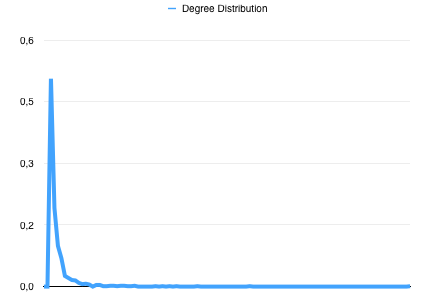
\includegraphics[scale=0.50]{img/dd-minimal-3-1000.png}
    %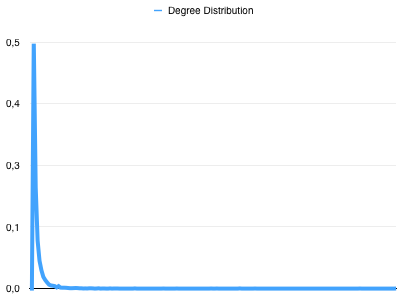
\includegraphics[scale=0.50]{img/dd-minimal-3-5000.png}
    
\end{figure}

\textbf{Comulative Degree Distribution}

\begin{figure}[h]
    \centering
    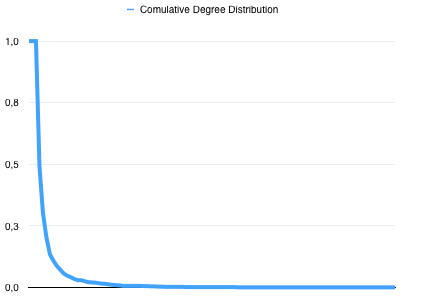
\includegraphics[scale=0.50]{img/cdd-minimal-3-1000.png}
    %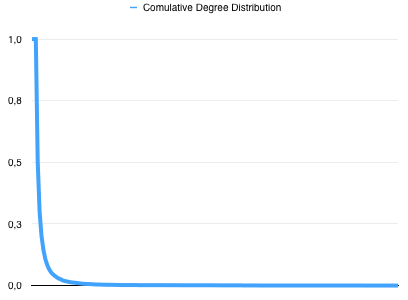
\includegraphics[scale=0.50]{img/cdd-minimal-3-5000.png}
    
\end{figure}

\begin{multicols}{2}

  \textbf{Clustering Coefficient}

  \textbf{(initial=3,nodes=1000)} 0,74002

  \textbf{(initial=3,nodes=5000)} ---

\columnbreak

  \textbf{Average Path Length}

  \textbf{(initial=3,nodes=1000)} 4,71825

  \textbf{(initial=3,nodes=5000)} ---

\end{multicols}

\begin{center}

  \textbf{Average degree: \textlangle k\textrangle}

  \textbf{(initial=3,nodes=1000)} 3.9940

  \textbf{(initial=3,nodes=5000)} 3.9988

\end{center}

\section{Conclusion and Data Analysis}
When gathering the results we noticed that it was taking too long to calculate the average path length for bigger graphs
(number of nodes up from 1000), so we changed the algorithm to find the shortest path. Even though we know that Bfs has a
time complexity of O(N²), for finding all the shortest distances on a graph it's better to use an algorithm such as Floyd Warshall,
which has a higher time complexity (O(N³)) but computes all the distances at once.

Analysing the random graph properties we can conclude that all the tests had the correct clustering coefficient, because it should
be the same as the probability of linking two nodes which was 0,05.

The average path length is also very similar to the theorical result, since the theorical \textlangle k\textrangle \ for both random graphs is:
$\frac{\ln1000}{\ln49.528}=1.77$ and $\frac{\ln5000}{\ln250.0884}=1.54$.
Both results don't differ too much from the average path lengths (2.031 and 1.949 respectively) and we can explain the difference by the randomization and the reduced size of the graphs used (compared to big systems).

Before implementing the minimal model we already knew that the theorical \textlangle k\textrangle \ was going to be aproximately 4. After the implementation and analysis we can confirm that result.

\section{Reference}
\begin{description}
  \item[Python] \href{https://www.python.org}{www.python.org}
  \item[networkx] \href{https://networkx.github.io}{networkx.github.io}
  \item[Lecture Slides]
  \item[Power Dataset] \href{https://github.com/gephi/gephi/wiki/Datasets#infrastructure-networks}{github.com/gephi/gephi/wiki/Datasets\#infrastructure-networks}
\end{description}

\end{document}
